\documentclass[12pt,a4paper]{ctexart}
\usepackage[margin=2.4cm]{geometry}
\usepackage{amsmath,amssymb}
\usepackage{graphicx}
\usepackage{booktabs}
\usepackage{array}
\usepackage{caption}
\usepackage{float}
\usepackage{hyperref}
\hypersetup{colorlinks=true,linkcolor=black,urlcolor=blue}
\setlength{\parskip}{0.4em}
\captionsetup{font=small,labelfont=bf}

\title{\bfseries 光电效应伏安特性与光强关系实验报告}
\author{姓名：\underline{\hspace{3cm}}\quad 学号：\underline{\hspace{3cm}}}
\date{\today}

\begin{document}
\maketitle

\begin{abstract}
测量光电管在不同入射光波长和不同光阑孔径下的伏安特性。实验中电压取 $-1\sim50\ \mathrm{V}$，将七组数据统一绘制于同一坐标系。结果表明，随正向电压增大，光电流先快速增加，随后增幅减小并逐渐趋于饱和。在波长 $404.7\ \mathrm{nm}$ 不变的条件下，以 $50\ \mathrm{V}$ 处电流近似表征饱和电流，$\Phi4$、$\Phi8$ 相对于 $\Phi2$ 的电流比分别为 $3.805$ 和 $15.390$，与光孔面积比 $4$ 和 $16$ 接近，说明饱和光电流与入射光强近似成正比。
\end{abstract}

\section{实验目的}
\begin{enumerate}
  \item 测量光电管的伏安特性，观察光电流随电压增加而趋于饱和的现象。
  \item 比较相同光阑孔径下不同波长入射光的伏安曲线。
  \item 在波长不变时研究光电流与光阑孔径的关系，检验饱和光电流与入射光强的正比关系。
\end{enumerate}

\section{实验原理}
光子能量为 $h\nu$。根据爱因斯坦光电效应方程，光电子的最大初动能满足
\begin{equation}
  \frac{1}{2}m v_{\max}^{2}=h\nu-W,
\end{equation}
其中 $h$ 为普朗克常量，$\nu=c/\lambda$ 为入射光频率，$W$ 为阴极材料的逸出功。当光子能量大于逸出功时，可以发生光电效应。

在正向电压较小时，并非所有光电子都能到达阳极，因此光电流随电压增加而明显增大。电压足够高后，阴极产生的光电子几乎都被阳极收集，电流逐渐达到饱和值 $I_s$。在入射光频率不变时，单位时间逸出的光电子数与入射光子数成正比，因而有
\begin{equation}
  I_s\propto P,
\end{equation}
其中 $P$ 为照射到阴极上的光功率。

若光源照明条件不变，通过圆形光阑的光功率与光阑面积成正比。设光阑直径为 $\Phi$，则
\begin{equation}
  P\propto S=\frac{\pi\Phi^{2}}{4},
  \qquad I_s\propto\Phi^{2}.
\end{equation}
所以，以 $\Phi2$ 为基准，$\Phi4$ 和 $\Phi8$ 对应的饱和电流理论比值分别为 $4$ 和 $16$。

\section{实验内容与数据处理}
实验记录分为两部分：
\begin{enumerate}
  \item 光阑为 $\Phi4$，分别采用 $365.0$、$404.7$、$577.0$ 和 $546.1\ \mathrm{nm}$ 的入射光，测量电压从 $-1\ \mathrm{V}$ 到 $50\ \mathrm{V}$ 时的电流。
  \item 入射光波长固定为 $404.7\ \mathrm{nm}$，分别采用 $\Phi2$、$\Phi4$ 和 $\Phi8$ 光阑，重复测量伏安特性。
\end{enumerate}
每次测量均改变电压并记录相应的电流示数，然后以电压为横坐标、电流为纵坐标作图。原始照片未标明电流单位，因此本文保留仪器示数，不自行换算电流单位。$\Phi4$、$404.7\ \mathrm{nm}$ 条件在两张照片中出现两次，本文将其作为两次独立测量保留，不进行平均。

\section{实验结果}
七组伏安曲线统一绘于图\ref{fig:all-data}。完整数值见附录表\ref{tab:raw-data}，同时保存于 \texttt{photoelectric\_data.csv}。

\begin{figure}[H]
  \centering
  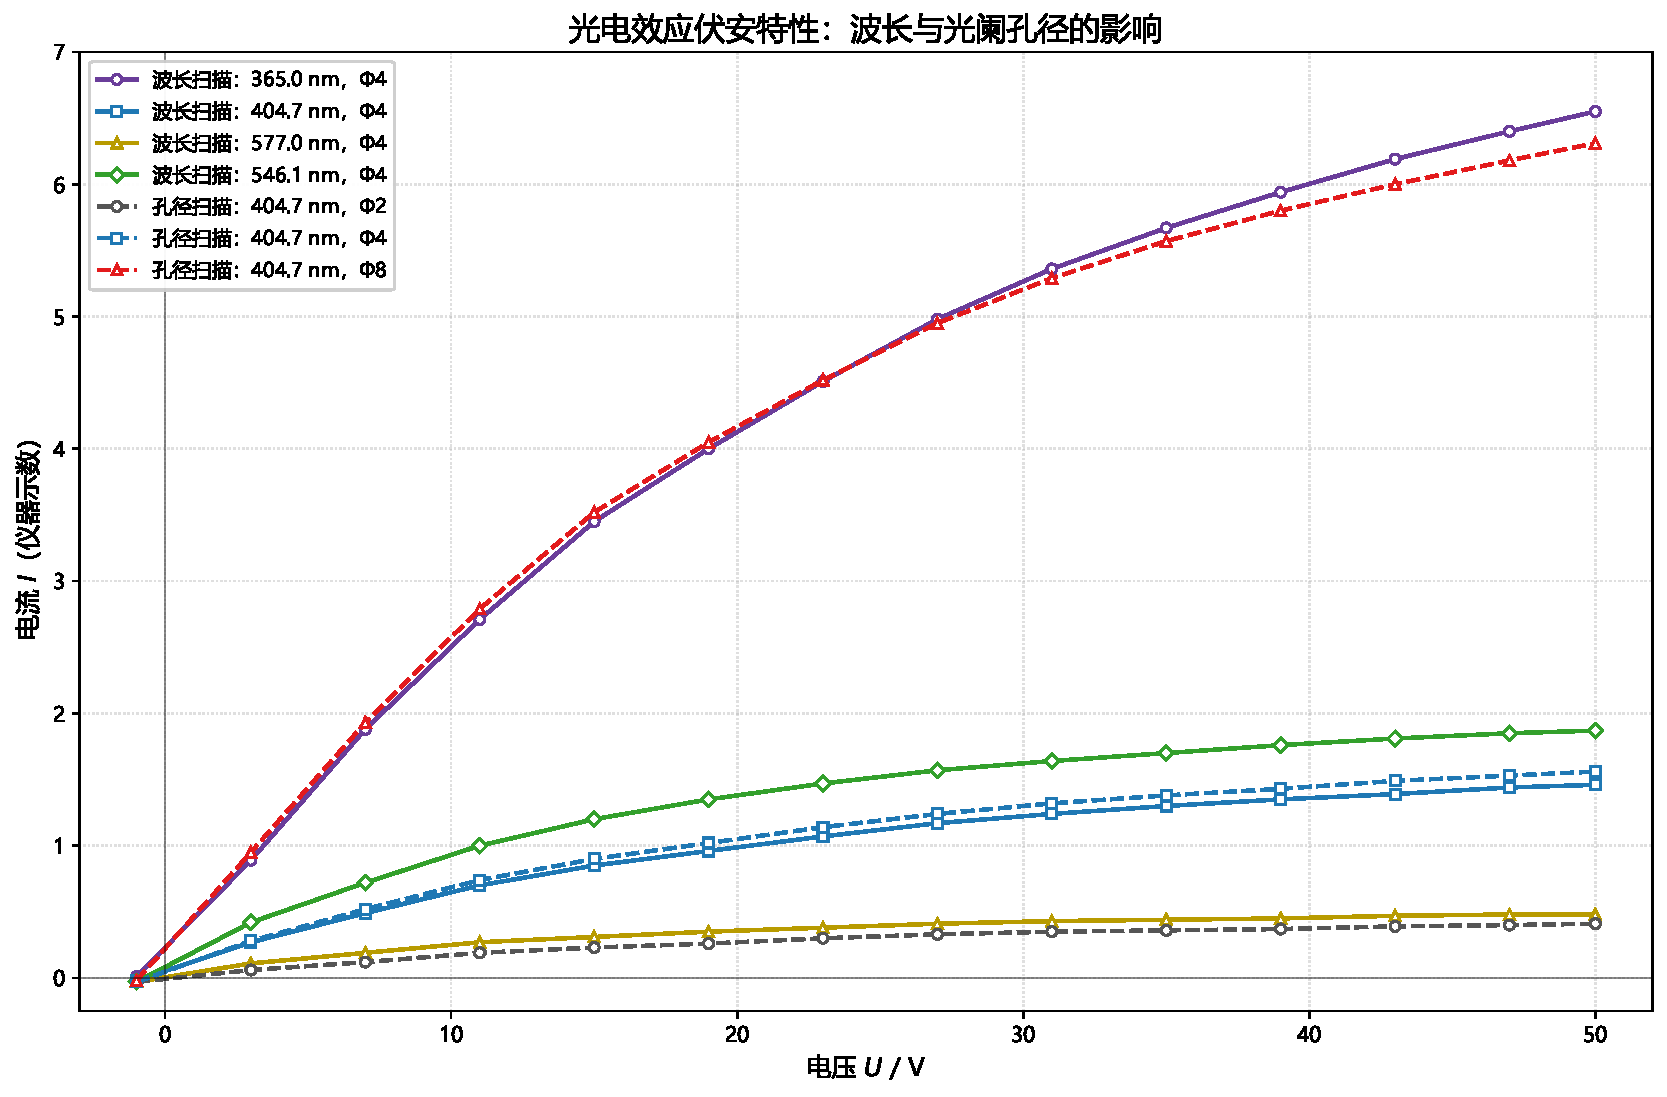
\includegraphics[width=0.98\textwidth]{photoelectric_all_data.pdf}
  \caption{不同波长及不同光阑孔径下的光电效应伏安特性}
  \label{fig:all-data}
\end{figure}

\subsection{伏安曲线的共同特征}
各组曲线均表现为低电压区增长较快、高电压区增长变慢。在 $30\sim50\ \mathrm{V}$ 范围内，多数曲线仍有小幅上升，说明实验电压范围内接近但未必完全达到饱和。因此，以下使用 $50\ \mathrm{V}$ 处的电流 $I_{50}$ 作为饱和电流的近似指标，而不是宣称其等于严格的饱和值。

在 $U=-1\ \mathrm{V}$ 时，各组示数接近零，部分读数约为 $-0.02\sim-0.03$。这些微小负值可能与仪器零点、暗电流或读数波动有关。

\subsection{不同波长下的曲线}
在相同 $\Phi4$ 条件下，$50\ \mathrm{V}$ 处的仪器示数分别为：$365.0\ \mathrm{nm}$ 时 $6.55$，$404.7\ \mathrm{nm}$ 时 $1.46$，$546.1\ \mathrm{nm}$ 时 $1.87$，$577.0\ \mathrm{nm}$ 时 $0.48$。各组均呈现逐渐饱和的趋势，但电流大小并不随波长单调变化。

饱和电流不仅取决于单个光子的能量，还取决于入射光强、光源光谱分布、滤光片透过率以及光阴极的光谱响应。因此，不能仅凭这四条曲线比较不同波长下的光子能量，也不能据此计算普朗克常量；后者还需要截止电压与频率的数据。

\subsection{光阑孔径与光电流的关系}
固定波长为 $404.7\ \mathrm{nm}$，三组光阑对应的 $50\ \mathrm{V}$ 电流示数如表\ref{tab:aperture}所示。

\begin{table}[H]
  \centering
  \caption{不同光阑孔径在 $50\ \mathrm{V}$ 处的电流及其比值}
  \label{tab:aperture}
  \begin{tabular}{ccccc}
    \toprule
    光阑 & $\Phi^2/\Phi_2^2$ & $I_{50}$（仪器示数） & $I_{50}/I_{50,\Phi2}$ & 相对面积比预期的偏差 \\
    \midrule
    $\Phi2$ & 1  & 0.41 & 1.000  & --- \\
    $\Phi4$ & 4  & 1.56 & 3.805  & $-4.88\%$ \\
    $\Phi8$ & 16 & 6.31 & 15.390 & $-3.81\%$ \\
    \bottomrule
  \end{tabular}
\end{table}

计算得
\begin{align}
  \frac{I_{50,\Phi4}}{I_{50,\Phi2}}&=\frac{1.56}{0.41}=3.805\approx4,\\
  \frac{I_{50,\Phi8}}{I_{50,\Phi2}}&=\frac{6.31}{0.41}=15.390\approx16.
\end{align}
实验比值与光阑面积比基本一致，支持饱和光电流与入射光强近似成正比的结论。两次 $\Phi4$、$404.7\ \mathrm{nm}$ 测量在 $50\ \mathrm{V}$ 处的示数分别为 $1.46$ 和 $1.56$，相对其平均值的差异约为 $6.6\%$，反映出一定的测量重复性差异。

\section{误差与讨论}
\begin{enumerate}
  \item 实验最高电压为 $50\ \mathrm{V}$，部分曲线尚未完全水平，以 $I_{50}$ 代替 $I_s$ 会引入近似误差。
  \item 光阑面积模型假定了照明空间分布、光源状态和光路条件不变；若照明不均匀或光路发生变化，实际光功率不再严格与 $\Phi^2$ 成正比。
  \item 仪器零点偏移、暗电流、光源波动以及读数分辨率都会影响低电流读数和不同测量轮次的一致性。
  \item 原始记录没有给出电流单位和仪器不确定度，故本文只比较同一仪器示数的比值，不给出绝对光电流及其不确定度。
\end{enumerate}

\section{结论}
实验得到的七组伏安曲线均显示：光电流随正向电压增加先较快上升，随后逐渐趋于饱和。固定 $404.7\ \mathrm{nm}$ 波长时，$\Phi4$ 和 $\Phi8$ 相对于 $\Phi2$ 的高电压端电流比分别为 $3.805$ 和 $15.390$，与光阑面积比 $4$ 和 $16$ 接近，偏差分别约为 $-4.88\%$ 和 $-3.81\%$。在实验误差和近似条件下，结果验证了饱和光电流与入射光强近似成正比。不同波长下的电流大小还受光强和光谱响应影响，不能仅依据本组伏安数据确定截止电压或普朗克常量。

\appendix
\section{原始实验数据}
\begin{table}[H]
  \centering
  \caption{七组实验的原始电流示数；$a$、$b$ 表示两次独立测量}
  \label{tab:raw-data}
  \small
  \begin{tabular}{c|cccc|ccc}
    \toprule
    & \multicolumn{4}{c|}{$\Phi4$，不同波长} & \multicolumn{3}{c}{$404.7\ \mathrm{nm}$，不同光阑} \\
    $U$/V & 365.0 nm & 404.7 nm$^a$ & 577.0 nm & 546.1 nm & $\Phi2$ & $\Phi4^b$ & $\Phi8$ \\
    \midrule
    $-1$ & 0.01 & $-0.02$ & $-0.03$ & $-0.03$ & $-0.03$ & $-0.03$ & $-0.02$ \\
    3  & 0.89 & 0.27 & 0.11 & 0.42 & 0.06 & 0.28 & 0.95 \\
    7  & 1.88 & 0.49 & 0.19 & 0.72 & 0.12 & 0.52 & 1.93 \\
    11 & 2.71 & 0.70 & 0.27 & 1.00 & 0.19 & 0.74 & 2.79 \\
    15 & 3.45 & 0.85 & 0.31 & 1.20 & 0.23 & 0.90 & 3.52 \\
    19 & 4.00 & 0.96 & 0.35 & 1.35 & 0.26 & 1.02 & 4.05 \\
    23 & 4.51 & 1.07 & 0.38 & 1.47 & 0.30 & 1.14 & 4.52 \\
    27 & 4.98 & 1.17 & 0.41 & 1.57 & 0.33 & 1.24 & 4.95 \\
    31 & 5.36 & 1.24 & 0.43 & 1.64 & 0.35 & 1.32 & 5.29 \\
    35 & 5.67 & 1.30 & 0.44 & 1.70 & 0.36 & 1.38 & 5.57 \\
    39 & 5.94 & 1.35 & 0.45 & 1.76 & 0.37 & 1.43 & 5.80 \\
    43 & 6.19 & 1.39 & 0.47 & 1.81 & 0.39 & 1.49 & 6.00 \\
    47 & 6.40 & 1.44 & 0.48 & 1.85 & 0.40 & 1.53 & 6.18 \\
    50 & 6.55 & 1.46 & 0.48 & 1.87 & 0.41 & 1.56 & 6.31 \\
    \bottomrule
  \end{tabular}
\end{table}

\end{document}
